\autsection{Camera}{Bhaaeddin Alhomsi}

The cameras will be triggered whenever a detects a flash of light, hopefully catching a glimpse of something living. CMOS camera sensor can detect the wavelength from 350 nm (UVA) till 1100 nm (IRA), so we have to find lighting source can cover this range .
Another approach that is developing very well is that of broad band fluorescence to very deep (short wavelength) ultraviolet (UV) light. The deep UV has the advantage that at such wavelengths there is very little background fluorescence, and it is easy to identify samples containing carbon-based chemistry that could be associated with life.
Infra-red light is radiated from any object with a temperature. Even objects which are too cool to be detected optically can be studied in the infra-red.
Panoramic image (360 degree) it will give us a good understanding how is the bottom of ice shield looks like.

\subsection{Lighting}

Ambient visible light is quickly attenuated by a combination of scattering and absorption, thus requiring artificial lighting to view items underwater with any degree of clarity. We see things in color because objects reflect wavelengths of light that represent the colors of the visible spectrum. Artificial lighting is therefore necessary near the illuminated object to view it in true color with intensity. Underwater lamps provide this capability.
Lamps convert electrical energy into light. The main types or classes of artificial lamps/light sources used in underwater lighting are incandescent, fluorescent, high intensity gas discharge, and light-emitting diode (LED) - each with its strengths and weaknesses. All types of light are meant to augment the natural light present in the environment.
 The flash lamps provide a short duration (about 0.005 see) heat pulse. The short burst of energy results in a momentary rise in the surface temperature of the part. The temperature rise may be detrimental to the top layer of the part being exposed. Therefore, it is necessary to ensure the non-destructive nature of the technique. Amount of the temperature rise determines whether the flash-lamp heating would be detrimental to the part. 
the flash duration is about 0.005 sec. Because of the short flash duration, relatively little amount of heat is imparted. The part temperature on the surface rises until end of the flash duration and then drops quickly due to the heat radiation and convection from the surface and the heat conduction into the part. The temperature rise on the part surface can be high enough to damage the top layer of the part.
The table below, shows the major types of artificial lighting systems, as well as their respective characteristics.
\begin{figure}[htb]
\centering
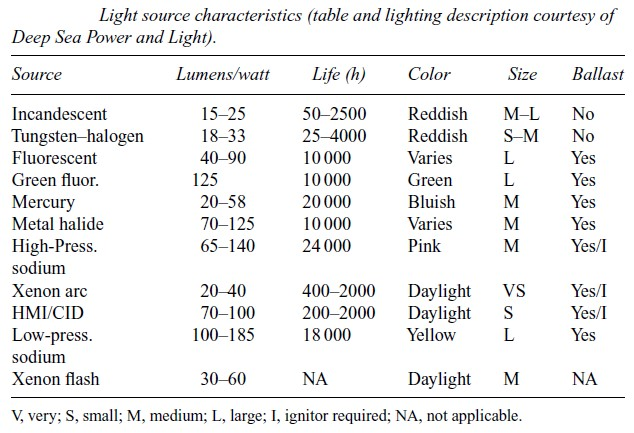
\includegraphics[scale=0.75]{figures/camera/bh6.jpg}
\caption{Light source characteristics}
\end{figure}
\\
Incandescent – The incandescent lamp was the first artificial light bulb invented.
Electricity is passed through a thin metal element, heating it to a high enough temperature to glow (thus producing light). It is inefficient as a lighting source with approximately 90 \% of the energy wasted as heat. Halogen bulbs are an improved incandescent. Light energy output is about 15 \% of energy input,  instead of 10 \%, allowing them to produce about 50 \% more light from the same amount of electrical power. However, the halogen bulb capsule is under high pressure instead of a vacuum or low-pressure noble gas (as with regular
incandescent lamps) and, although much smaller, its hotter filament temperature causes the bulbs to have a very hot surface. This means that such glass bulbs can explode if broken, or if operated with residue (such as fingerprints) on them. The risk of burns or fire is also greater than other bulbs, leading to their prohibition in
some underwater applications. Halogen capsules can be put inside regular bulbs or dichroic reflectors, either for aesthetics or for safety. Good halogen bulbs produce a sunshine-like white light, while regular incandescent bulbs produce a light between sunlight and candlelight.
\begin{figure}[htb]
\centering
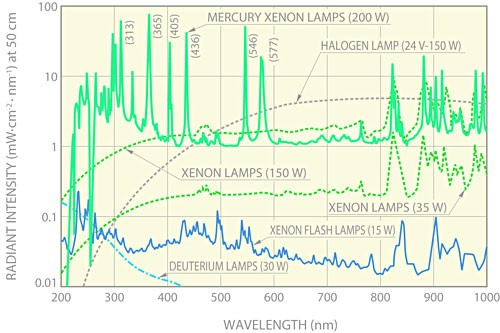
\includegraphics[scale=1]{figures/camera/bh7.jpg}
\caption{Lamp wavelength}
\end{figure}
\\
A fluorescent lamp is a type of lamp that uses electricity to excite
mercury vapour in argon or neon gas, producing short-wave ultraviolet light. This
light then causes a phosphor coating on the light tube to fluoresce, producing
visible light. Fluorescent bulbs are about 40 \% efficient, meaning that for
the same amount of light they use one-fourth the power and produce one-sixth the
heat of a regular incandescent. Fluorescents typically do not have the luminescent
output capacity per unit volume of other types of lighting, making them (in many
underwater applications) a poor choice for underwater artificial light sources.

High-intensity discharge – High-intensity discharge (HID) lamps include the
following types of electrical lights: Mercury vapour, metal halide, high pressure
sodium and, less common, xenon short-arc lamps. The light-producing
element of these lamp types is a well-stabilized arc discharge contained within
a refractory envelope (arc tube) with wall loading (power intensity per unit area
of the arc tube) in excess of 3W/cm2 (19.4 W/in2). Compared to fluorescent
and incandescent lamps, HID lamps produce a large quantity of light in a small
package, making them well suited for mounting on underwater vehicles. The
most common HID lights used in underwater work are of the metal halide type.

LED – A light-emitting diode (LED) is a semiconductor device that emits incoherent
narrow-spectrum light when electrically biased in the forward direction.
This effect is a form of electroluminescence. The color of the emitted light
depends on the chemical composition of the semiconducting material used,
and can be near-ultraviolet, visible, or infra-red. LED technology is useful for
underwater lighting because of its low power consumption, low heat generation,
instantaneous on/off control, continuity of color throughout the life of the diode,
extremely long life, and relatively low cost of manufacture. LED lighting is a
rapidly evolving technology.

We will select xenon lamp 150 W, because it will provide us with good radiant intensity for the whole wavelength range.

\subsection{Reflector}

An efficient reflector will not only maximize the light output that falls on the target,
but will also direct heat forward and away from the lamp. The shape of the reflector
will be the main determinant in how the light output is directed. Most are parabolic,
but ellipsoidal reflectors are often used in underwater applications to focus light
through a small opening in a pressure housing. The surface condition of a reflector
will determine how the light output will be dispersed and diffused. The majority of
reflectors are made of pure, highly polished aluminium that will reflect light back at
roughly the same angle to the normal at which it was incident. By adding dimples or
peens to the surface, the reflected light is dispersed or spread out. When a plain white surface is used, the reflected light is diffused in all directions.

\subsection{The wavelength range of optical radiation}

The term "optical radiation" refers to electromagnetic radiation in the wavelength range between 100 nm and 1 mm. The terms "light" and "visible radiation" (VIS) refer to the wavelength range between 400 nm and 800 nm, which can be perceived by the human eye. Optical radiation with wavelengths shorter than 400 nm is called ultraviolet (UV) radiation and is further subdivided in UV-A, UV-B and UV-C ranges. Similarly, infra-red (IR) radiation covers the wavelength range above 800 nm and is subdivided in IR-A, IR-B and IR-C ranges.

\begin{figure}[htb]
\centering
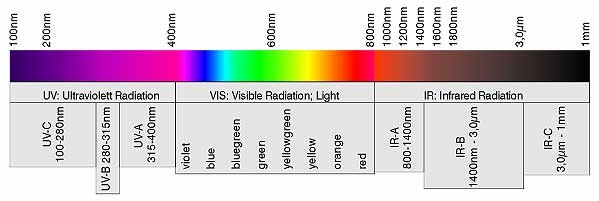
\includegraphics[scale=1]{figures/camera/bh8.jpg}
\caption{The wavelength range of optical radiation}
\end{figure}

The sensitivity of the human eye to light of a certain intensity varies strongly over the wavelength range between 380 and 800 nm. Under daylight conditions, the average normal sighted human eye is most sensitive at a wavelength of 555 nm.

\subsection{Camera}

The ECAM imaging system delivers cost-effective, short lead-time, high-performance, and reliable space imaging as a modular off-the-shelf solution. The C50 utilizes a CMOS image sensor with integral RGB Bayer Pattern color filter array. The sensor outputs 10-bit pixels that are square-root companded to 8-bits before being transmitted to the DVR on a 200 Mbit/s serial link.. Preprocessing typically includes Bayer Pattern interpolation and direct conversion to the YCbCr color space using a 5 x 5 filter kernel. The video is also reformatted as needed for input to either a JPEG (lossy) or Huffman First Difference (lossless) compressor. The C50 is highly configurable. The exposure and gain may be adjusted to support widely varying scene.
The optical lens made of a material that has substantially the same index of refraction as that of water.

\begin{figure}[htb]
\centering
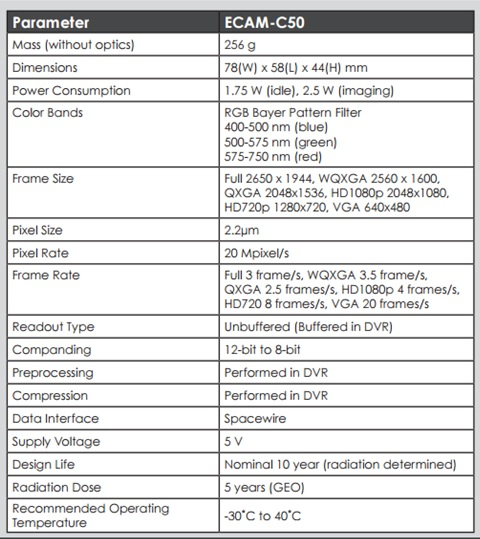
\includegraphics[width=.48\textwidth]{figures/camera/bh10.jpg}
\caption{Camera parameters}
\end{figure}

CMOS sensor can detect the wavelength from 350 nm (UVA) till 1100 nm (IRA), so we have to find lighting source can cover this range .

\begin{figure}[htb]
\centering
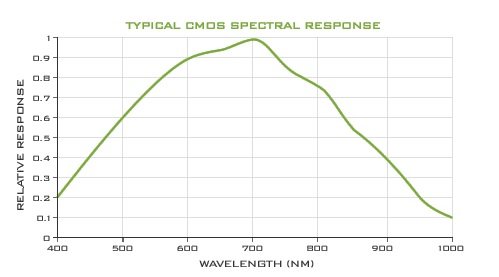
\includegraphics[scale=1]{figures/camera/bh9.jpg}
\caption{CMOS spectral response}
\end{figure}

\subsection{Panoramic Images}

To take a panorama, the camera is rotated at fixed angular increments, taking an image at each point. These images can then be assembled (stitched) using stitching software, which allows the images to be aligned and combined into a single seamless panoramic image, either automatically (using image analysis) or manually (with user supplied control points). The final panoramic image can then be viewed or printed as a flat image or viewed interactively using specific playback software.
The rotation angle depend on camera field of view , in or proposed camera the field of view angle is approximately 70 degree , so to build 360 panoramic image we need 5 photos with rotation angle 70 degree between each shoot.
Robotic panoramic heads are also available. The robotic head performs the rotation and image capture functions automatically under computer control. Robotic heads can also be used with time-lapse photography.
